\documentclass[letter,10pt]{article}
\usepackage[utf8]{inputenc}
\usepackage[spanish, activeacute]{babel}
\usepackage{geometry}
\geometry{verbose,tmargin=0cm,bmargin=2cm,lmargin=2cm,rmargin=2cm,headheight=0cm,headsep=1cm,footskip=1cm}
\usepackage{graphicx}
\usepackage{fancyhdr}
\pagestyle{fancy}
\cfoot{10}

%%%%%%%%%%%%%%%%%%%%%%%%%%%%%% Textclass specific LaTeX commands.
\newcommand{\lyxaddress}[1]{
\par {\raggedright #1
\vspace{1.4em}
\noindent\par}
}

%%%%%%%%%%%%%%%%%%%%%%%%%%%%%% User specified LaTeX commands.
\date{}

\begin{document}

\title{Problema A - A ? B}


\includegraphics[scale=0.6]{logo} \hspace*{9.00cm}

\includegraphics[scale=0.5]{dsc} 
\bigskip
\begin{center}
    \Large Problema I - Investigando laberintos
\end{center}

\begin{flushright}
Límite de tiempo: 3 segundos
\par\end{flushright}
\bigskip

\section*{Problema}

Un laberinto es representado en una cuadrídula de dos dimensiones como está ilustrado en la figura siguiente. 

\begin{center}
    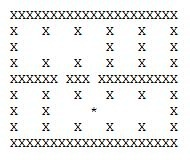
\includegraphics{1.jpg}
\end{center}


Cada punto de la cuadrícula es representado por un carácter. Un carácter espacio (`$ $') representa los lugares en dónde puedes caminar.

Las paredes del laberinto son representadas por letras mayúsculas (de 'A' a 'Z'), esto es, lugares dónde no puedes caminar.


Tu tarea es, dado un punto de inicio dentro del laberinto, representado por un asterisco ('*'), debes de marcar todos los posibles lugares a dónde puedes llegar caminando con el carácter gato ($'$$#$$'$). El asterisco debe ser reemplazado por el carácter gato.


La forma en que puedes caminar es 4 conexidad, esto significa que solo puedes moverte hacia arriba, abajo, izquierda o derecha.

La cuadricula presentada anteriormente quedaría:

\begin{center}
    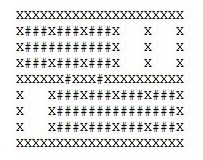
\includegraphics{2.jpg}
\end{center}


$$$$$$$$$$$$$$$$$$$$$$$$$$$$$$$$$$$$$$$$$$
$$
\cfoot{11}
\subsection*{Entrada}

La primera línea de entrada es T, el número de casos. La primera línea de cada caso son dos enteros, $N$ y $M$, el número de renglones y el número de columnas de la cuadrícula respectivamente.

Las siguientes $N$ lineas contienen $M$ carácteres, las cuales representan al laberinto.


\subsection*{Salida}

N líneas de M carácteres cada una, las cuales representa a la cuadrícula marcada en la forma en que se indicó.

Imprime una línea en blanco al final de cada caso.



\subsection*{Entrada Ejemplo}
\begin{verbatim}
2
5 5
XXXXX
X*  X
X   X
XX XX
XXXXX
5 9
AAAAAAAAA
C*  D   B
C   D   B
C   D   B
EEEEEEEEE
\end{verbatim}

\subsection*{Salida Ejemplo}

\begin{verbatim}
XXXXX
X###X
X###X
XX#XX
XXXXX

AAAAAAAAA
C###D   B
C###D   B
C###D   B
EEEEEEEEE

\end{verbatim}

\noindent \rule[0.5ex]{1\columnwidth}{1pt}


\lyxaddress{Maximiliano Vera Luna - Grupo de Algoritmia Avanzada y Programación Competitiva}
\end{document}
